\section{Chapter Overview}
This chapter contains details of the measurements carried out on networks of various sizes and investigation into the impact of a number of decisions made in the design process. Explanations will be given or analysis made of the results, which will be given in the form of of either plots or tables, depending on which allows for more concise presentation of the data. Both 2x2 and 3x3 network performance analysis was performed with no input delay to the \ac{LF}, which Section \ref{subsection:lf_delay} will show to have a significant performance impact. All tests were carried out, unless otherwise stated, at a centre frequency of $5~\si{\mega\hertz}$.

\section{2x2 Network Performance Comparison}
In order to investigate the impact of the \ac{ADPLL} network on performance, and conversely the impact of each individual \ac{ADPLL} design on the network, switches were used to alter the configuration of the network without requiring re-implementation and a number of captures made at each setting. The three configurations were: each \ac{ADPLL} individually locked to the reference, the network in uni-directional mode and bi-directional mode. The centre frequency or gains were not changed between measurements in order to obtain a good comparison. For \ac{ADPLL} 1 the gains were: $k_p = \frac{1}{32}$ \& $k_i = \frac{1}{256}$. For \ac{ADPLL} 2 and 3 they were: $k_p = \frac{1}{16}$ \& $k_i = \frac{1}{64}$. The

There are two main trends worth highlighting here, with the first of these being as the feedback network becomes more complicated a large degree of skew is introduced, with the magnitude becoming larger in the \acp{ADPLL} further from the reference. This would appear to be attributable to a combination of the time taken for a change in the reference to propagate to the \ac{ADPLL} node in question, and the fineness of period and detection resolutions. This second observation follows from the significant reduction in the skew growth in Designs 2 \& 3 which have finer resolutions.

The other trend, is the variation in \ac{C2C} jitter across the \ac{ADPLL} designs, with coarseness of the \ac{FPGA} clocked \ac{DCO} becoming somewhat obvious. As free \aclp{PLL} (\acsp{PLL}), the clocked \ac{DCO} has almost identical \ac{C2C} jitter and maximum \ac{TIE}, implying that only two period steps are used the majority of the time. As these steps are somewhat further apart than that of the \ac{RO}, at $3.875~\si{\nano\second}$ apart as opposed to an implementation dependant value in the region of $1.1765~\si{\nano\second}$, a much greater jitter is observed. This would confirm the belief that the \ac{FPGA} clocked designs are better suited to operational frequencies where the generated clock period to \ac{FPGA} clock period ratio is significantly lower than the $\frac{3.875~\si{\nano\second}}{200~\si{\nano\second}} = \frac{1}{51.6}$ in this design. Comparing the \ac{C2C} jitter of \ac{ADPLL} 1 \& 2, where the main difference is the choice of \ac{PFD}, the approximate $\frac{1.6~\si{\nano\second}}{0.50~\si{\nano\second}} \approx 3.2$ ratio of observed jitters is almost identical to the $\frac{3.875~\si{\nano\second}}{1.1765~\si{\nano\second}} \approx 3.29$ ratio of the period steps at $5~\si{\mega\hertz}$, implying the \ac{PFD} is at fault for this difference.

The other notable difference in \ac{C2C} jitter, is that the use of an inverter based \ac{TDC}, and its accompanying variation due to implementation differences, has the expected result of additional \ac{C2C} jitter, however, this impact is signfiicantly less than the that of changes in the \ac{RO} period step, and the inverter based \ac{TDC} in combination with the \ac{FPGA} clocked \ac{DCO} would still suffer the same problems as it does in \ac{ADPLL} Design 1 with the clocked \ac{PFD}.

%TODO additional comments with new data?

\begin{table}[!ht]
    \begin{center}
        \begin{footnotesize}
            \setlength{\tabcolsep}{.9\tabcolsep}
            \begin{tabular}{ll|r|r|r|r|r|r|r|r|r|}           
                \cline{3-11}
                && \multicolumn{3}{c|}{Jitter Standard Deviation (ns)} & \multicolumn{3}{c|}{Max. Time Interval Error (ns)} & \multicolumn{3}{c|}{Skew (ns)} \T\\
                \cline{3-11} 
                &&PLL 11&PLL 12&PLL 22    &PLL 11&PLL 12&PLL 22    &PLL 11&PLL 12&PLL 22\T\\
                \hline
                \multicolumn{2}{|l|}{\ac{ADPLL} Design 1}&-&-&-&-&-&-&-&-&-\T\\
                \multicolumn{2}{|r|}{Free PLLs} &1.6051  &1.6146  &1.6251     &1.6985 &1.5833 &1.2712    &0.2700 &0.5817 &0.2491 \T\\
                \multicolumn{2}{|r|}{Uni-dir.}  &1.7693  &1.8463  &1.8862     &7.3060 &7.2565 &10.151    &2.2791 &1.2822 &1.6299 \T\\
                \multicolumn{2}{|r|}{Bi-dir.}   &1.9964  &1.9146  &1.9572     &15.089 &18.283 &19.673    &9.2449 &11.612 &12.052 \T\\
                \hline
                \multicolumn{2}{|l|}{\ac{ADPLL} Design 2}&-&-&-&-&-&-&-&-&-\T\\
                \multicolumn{2}{|r|}{Free PLLs} &0.56222 &0.49224 &0.64124    &5.3039 &7.8626 &5.4634    &&& \T\\
                \multicolumn{2}{|r|}{Uni-dir.}  &0.55040 &0.51284 &0.62796    &5.5312 &7.5359 &7.9697    &&& \T\\
                \multicolumn{2}{|r|}{Bi-dir.}   &0.57056 &0.50403 &0.61644    &11.515 &15.943 &17.428    &&& \T\\
                \hline
                \multicolumn{2}{|l|}{\ac{ADPLL} Design 3}&-&-&-&-&-&-&-&-&-\T\\
                \multicolumn{2}{|r|}{Free PLLs} &0.66757 &0.84477 &0.71308    &5.9142 &6.1353 &5.3939    &-0.36997 &-0.20981 &-1.3344  \T\\
                \multicolumn{2}{|r|}{Uni-dir.}  &0.66934 &0.83894 &0.71271    &5.8779 &7.1746 &6.8914    &-0.36645 &-0.05647 &-0.36178 \T\\
                \multicolumn{2}{|r|}{Bi-dir.}   &0.68372 &0.83193 &0.68570    &7.5705 &9.6292 &9.7715    & 0.68901 & 1.58720 & 1.5553  \T\\
                \hline
                \B                
            \end{tabular}
        \end{footnotesize}
        \caption{2x2 Network performance Comparison.}
        \label{table:2x2perf}
    \end{center}
    \vspace{-0.5cm}
\end{table}
%\FloatBarrier

\section{3x3 Network Performance Comparison}
Subsequent to tests carried out using a 2x2 network, the corresponding tests were carried out using a 3x3 network in order to analyse the impact of a larger network. For these tests the gains were left unchanged but, as the 2x2 and 3x3 networks have different floorplans, the \acp{RO} have changed somewhat. This has especially manifested itself in the exceptional individual \ac{PLL} performance of Design 3.

From analysis of the 2x2 network, it was evident that the best performing design was going to be \ac{ADPLL} 3, as both \ac{ADPLL} 2 \& 3 contain the clocked \ac{PFD} which appears to cause significant skew as the \ac{ADPLL} node indices increase and move further from the external reference. The increased network size appears to have made the lag between reference edge and the rising edges of the individual generated signals worse, which would be expected as the number of clock cycles required to respond to a change in the phase relationship between reference and the furthest node has increased. \ac{ADPLL} 3 suffers least from the greater complication of the network, likely as a result of its period and detector resolution being the finest of the three designs considered.

As \ac{ADPLL} Design 1 suffered significantly more with skew as the node indices increased, so it is no surprise that in the larger network the problem has been amplified, meaning this design is not well suited for use in larger networks at this frequency due to poor resolution. This does not, however, impact the main role of this design method, which is the emulation of designs intended for use in \aclp{ASIC} (\acsp{ASIC}) as the frequency of operation will be much lower than the $5~\si{\mega\hertz}$ used in these tests, which will bring with it a finer resolution.
%TODO fill in this after measurements
\begin{table}[!ht]
    \begin{center}
        \begin{footnotesize}
            \setlength{\tabcolsep}{.9\tabcolsep}
            \begin{tabular}{ll|r|r|r|r|r|r|r|r|r|}           
                \cline{3-11}
                && \multicolumn{3}{c|}{Jitter Standard Deviation (ns)} & \multicolumn{3}{c|}{Max. Time Interval Error (ns)} & \multicolumn{3}{c|}{Skew (ns)} \T\\
                \cline{3-11} 
                &&PLL 11&PLL 12&PLL 22    &PLL 11&PLL 12&PLL 22    &PLL 11&PLL 12&PLL 22\T\\
                \hline
                \multicolumn{2}{|l|}{\ac{ADPLL} Design 1}&-&-&-&-&-&-&-&-&-\T\\
                \multicolumn{2}{|r|}{Free PLLs} &&& &&& &&& \T\\
                \multicolumn{2}{|r|}{Uni-dir.}  &&& &&& &&& \T\\
                \multicolumn{2}{|r|}{Bi-dir.}   &&& &&& &&& \T\\
                \hline
                \multicolumn{2}{|l|}{\ac{ADPLL} Design 2}&-&-&-&-&-&-&-&-&-\T\\
                \multicolumn{2}{|r|}{Free PLLs} &0.47167 &0.55012 &0.36251    &5.9649 &6.6965 &5.5010    &3.4045&3.2369&2.3108 \T\\
                \multicolumn{2}{|r|}{Uni-dir.}  &0.49292 &0.55586 &0.39054    &5.958  &8.9250 &11.622    &3.5052&6.9860&8.874 \T\\
                \multicolumn{2}{|r|}{Bi-dir.}   &0.43263 &0.48053 &0.33778    &18.867 &35.973 &38.773    &15.193&28.965&30.841 \T\\
                \hline
                \multicolumn{2}{|l|}{\ac{ADPLL} Design 3}&-&-&-&-&-&-&-&-&-\T\\
                \multicolumn{2}{|r|}{Free PLLs} &0.89042 &0.64889 &0.57405    &4.0634 &3.2467 &2.3141    &1.8373&1.1006&0.39334 \T\\
                \multicolumn{2}{|r|}{Uni-dir.}  &0.93580 &0.93353 &0.71361    &4.2675 &5.8193 &6.4139    &1.8605&2.3172&3.1463  \T\\
                \multicolumn{2}{|r|}{Bi-dir.}   &0.97717 &0.85131 &0.63863    &5.6439 &8.4856 &9.4467    &2.7129&4.1074&5.1717  \T\\
                \hline
                \B                
            \end{tabular}
        \end{footnotesize}
        \caption{3x3 Network performance Comparison.}
        \label{table:3x3perf}
    \end{center}
    \vspace{-0.5cm}
\end{table}
%\FloatBarrier

\section{Minor Variations}\label{section:minor_variations}
A number of minor design decisions will be tested in this section against their alternatives, as will the impact of varying the \ac{LF} gains.

\subsection{Impact of Gain Variation}
The gains chosen for use in the \acl{LF} have significant impact on the performance of the system, as the \ac{LF} governs the response of the \ac{ADPLL} to a given phase error. To large a proportional gain will result in overly aggressive overcompensation, thus negatively affecting the jitter. Eventually the violence of the jitter will result in a loss of lock. However, if the gain is too small, the frequency or period adjustment will not be sufficiently large to cause the \ac{ADPLL} to lock. Similarly, appropriate values of $k_i$ are required, and the relationship between proportional and integral gains must satisfy the conditions set out by Koskin \cite{koskin2018generation}.

\begin{figure}[h]
    \centering
    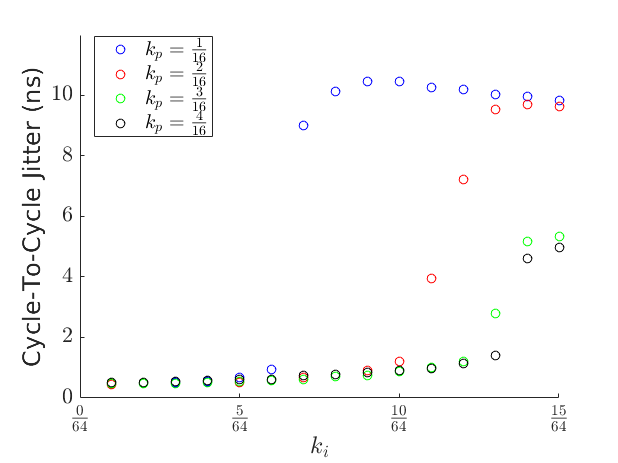
\includegraphics[width=0.6\textwidth]{../fixed_kp.png}
    \caption[Fixed $k_p$ integral gain sweeps]{Fixed $k_p$ integral gain sweeps.}
    \label{fig:gain_sweep}
\end{figure}
\begin{figure}[h]
    \centering
    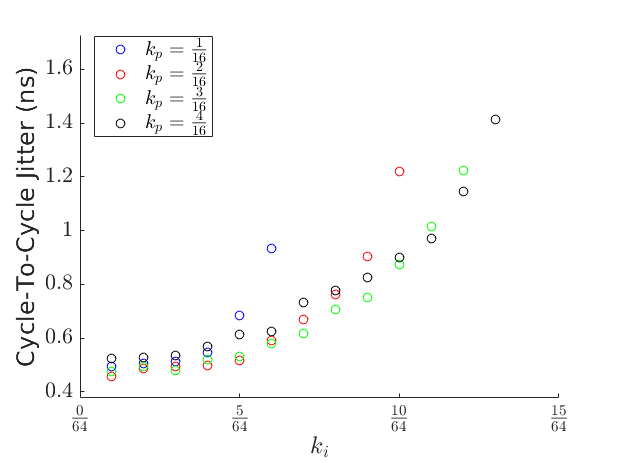
\includegraphics[width=0.6\textwidth]{../fixed_kp_zoom.png} 
    \caption[Fixed $k_p$ integral gain sweeps]{Fixed $k_p$ integral gain sweeps.}
    \label{fig:gain_sweep_zoom}
\end{figure}

Figure \ref{fig:gain_sweep} contains a sweep across the possible range of integral gains for four different proportional gains. This test was carried out with a 3x3 network of \ac{ADPLL} Design 3, each locked to the external reference at $5~\si{\mega\hertz}$, and the generated waveform from the \acp{ADPLL} at locations ``11'', ``22'' and  ``33'' were captured. It can clearly be observed that there are two distinct regions in the graph, with jitter values of less than $1~\si{\nano\second}$ contrasting sharply with the points with jitter in the region of $10~\si{\nano\second}$. These distinct sections of the plot represent locked and unlocked operation respectively. Zooming in on the low jitter region in Figure \ref{fig:gain_sweep_zoom}, the approximate loss of lock thresholds can be compared with the theoretical relationship of $k_i = 0.5\times k_p$. The approximated loss of lock is determined as gain setting that caused the first \ac{ADPLL} to lose lock.
\begin{table}[!h]
    \begin{center}
        \begin{tabular}{lrr}
            \multicolumn{1}{c}{$k_p$} & \multicolumn{1}{c}{$k_i$} & \multicolumn{1}{c}{Ratio} \T\B\\
            \hline
            $\frac{1}{16}$            & $\frac{5}{64}$            & $0.8$ \T\B\\
            $\frac{2}{16}$            & $\frac{11}{64}$           & $0.72$ \T\B\\
            $\frac{3}{16}$            & $\frac{13}{64}$           & $0.92$ \T\B\\
            $\frac{4}{16}$            & $\frac{15}{64}$           & $1.07$ \T\B
        \end{tabular}
    \end{center}
    \vspace{-0.5cm}
    \caption[Loss of Lock Gains]{Loss of Lock Gains.}
    \label{table:lolgains}
\end{table}

Despite the relatively small number of proportional gains, it is clear that the relationship set out by Koskin does not hold in this system, but rather a scaled version of it.  This difference is attributable to a difference in \ac{LF} structure. In his simulations the \ac{LF} design contains a register forming an input buffer, absent in the \ac{LF} used for these tests. The presence of this register, clocked on the generated signal, causes the \ac{ADPLL} to react more slowly to changes in the phase difference, thus increasing the jitter. The removal of this register causes a change in the relationship between proportional and integral gains, a change that will be investigated further in a later section.

\subsection{Distribution of Period Steps}
To add context to the jitter numbers produced for each oscillator previously, the variation of period steps in the \ac{RO}, and delays in the \ac{TDL} due to implementation should be examined. The best way to visualise this distribution is through a histogram, placing periods of in a certain range into the same bin. This can be visualised effectively using Matlab's \texttt{histplot}. In order to obtain data, three \acp{ADPLL} implementing both the \ac{FPGA} clocked and inverter based \acp{DCO} were locked to an external reference signal at $5~\si{\mega\hertz}$, and the period of each clock cycle measured.
\begin{figure}[h]%
    \centering
    \subfloat[Inverter propagation delay based \ac{RO}.]{{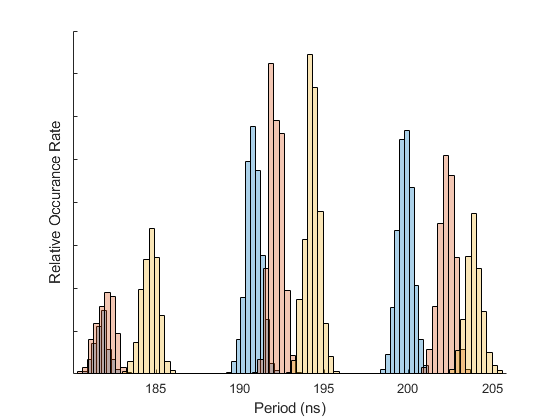
\includegraphics[width=0.5\textwidth]{../conf_paper/distrib_ring} }}%
    \subfloat[\ac{FPGA} clocked \ac{DCO}.]{{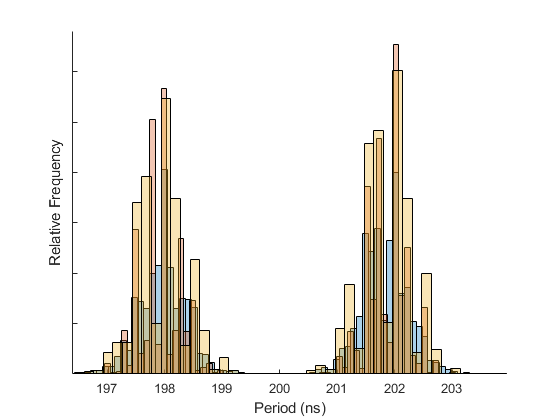
\includegraphics[width=0.5\textwidth]{../conf_paper/distrib_pa} }}%
    \caption[Example distribution of periods]{Example distribution of periods.}    
    \label{fig:dists}
\end{figure}
Figure \ref{fig:dists} contains the output of \texttt{histfit} for each of the three oscillators superimposed in one plot for each \ac{DCO} type. As the \ac{RO} has significantly finer period resolution, the period steps would be overlaid on each-other thereby making the plot difficult to read. In order to avoid this behaviour, the \ac{RO}'s mapping of control code to inverters to remove was altered from twice the control code to 16 times the control code. This results in a more pronounced separation of period steps while being indicative of the variation due to implementation.
The plots paint a a picture of the unrealistic nature of the \ac{FPGA} clocked design in comparison to its inverter based counterpart, as each oscillator will have identical intrinsic period steps thus eliminating any jitter that maybe be seen in the system due to misalignment.
This effects the suitability of the FPGA clocked \ac{DCO} for the improvement of simulation models, or the examination of how a novel block may impact the behaviour of the network. If this analysis was carried out for the period steps, similar behaviour would be observed.


\subsection{\ac{FPGA} Clocked \ac{DCO} Width Variation}
When introducing the design of the \ac{DCO} for \ac{ADPLL} 1, the minimum possible accumulator width was chosen. From the equation used to calculate the frequency step size, it may have seemed that by doubling the bias point and increasing the width of the counter to 13 bits a finer resolution could be achieved.
\begin{align}
f_{step} &= \frac{f_{FPGA}}{2^{12}} = 62.988~\si{\kilo\hertz} \\
f_{step} &= \frac{f_{FPGA}}{2^{13}} = 31.494~\si{\kilo\hertz}
\end{align}
As Table \ref{table:accum_width} shows, this is not in fact the case. Both measurements were carried out using identical loop filter gains, network configurations and reference signal. While in uni-directional mode some difference is observed in the maximum \ac{TIE}, but in all other aspects no statistically relevant changes can be seen.
%TODO explanation for this?
\begin{table}[!ht]
    \begin{center}
        \begin{footnotesize}
            \setlength{\tabcolsep}{.9\tabcolsep}
            \begin{tabular}{ll|r|r|r|r|r|r|r|r|r|}           
                \cline{3-11}
                && \multicolumn{3}{c|}{Jitter Standard Deviation (ns)} & \multicolumn{3}{c|}{Max. Time Interval Error (ns)} & \multicolumn{3}{c|}{Skew (ns)} \T\\
                \cline{3-11} 
                &&PLL 11&PLL 12&PLL 22    &PLL 11&PLL 12&PLL 22    &PLL 11&PLL 12&PLL 22\T\\
                \hline
                \multicolumn{2}{|l|}{Accum. Width 12}&-&-&-&-&-&-&-&-&-\T\\
                \multicolumn{2}{|r|}{Uni-dir.}  &1.7693 &1.8463 &1.8862    &7.3060  &7.2565  &10.151    &2.2791 &1.2822  &1.6299  \T\\
                \multicolumn{2}{|r|}{Bi-dir.}   &1.9964 &1.9146 &1.9572    &15.0890 &18.2830 &19.673    &9.2449 &11.6120 &12.0520 \T\\
                \hline
                \multicolumn{2}{|l|}{Accum. Width 13}&-&-&-&-&-&-&-&-&-\T\\
                \multicolumn{2}{|r|}{Uni-dir.}  &1.7946 &1.8161 &1.9048    &6.8614  &7.1495 &9.371      &2.2257 &1.6328  &1.3778  \T\\
                \multicolumn{2}{|r|}{Bi-dir.}   &2.0016 &1.9217 &1.9605    &14.9580 &18.938 &19.510     &9.1678 &12.0000 &11.7690 \T\\
                \hline
                \B
            \end{tabular}
        \end{footnotesize}
        \caption{\ac{DCO} Accumulator Width Comparison.}
        \label{table:accum_width}
    \end{center}
    \vspace{-0.5cm}
\end{table}
%\FloatBarrier

\subsection{\ac{LF} Input Delay Register}\label{subsection:lf_delay}
Previously, when comparing the loss of lock gain relationship to that proposed by Koskin \textit{et al}, it was mentioned that the \ac{LF} used in this project does not have an input delay register. The lack of agreement between the theory and experimental results was attributed to the input delay register, or lack thereof. In order to provide a basis for this claim, the performance of a network in 2x2 configuration, was analysed and the results of this analysis are presented in Table \ref{table:lf_delay}. While the \ac{C2C} jitter is statistically similar, there is significant different to be observed in the \ac{TIE}, where an approximately $50\%$ increase can be observed, measurement for measurement. As the maximum \ac{TIE} is significantly impacted by the presence of any skew, as skew is the average value of this difference, it is interesting to note that the relationship is in fact the opposite. It is in precisely this situation that \ac{C2C} jitter as a measurement is non-ideal. \ac{C2C} jitter does not differentiate between the situations in which while the period variation might be the same for multiple clock cycles in the same or opposite directions. As the extra cycle of delay due to the input register increases the reaction time of the \ac{ADPLL} to any changes, the delay between clock edges increases. \ac{TIE} is, however, affected by this difference which can be clearly seen in the table.

\begin{table}[!ht]
    \begin{center}
        \begin{footnotesize}
            \setlength{\tabcolsep}{.9\tabcolsep}
            \begin{tabular}{ll|r|r|r|r|r|r|r|r|r|}           
                \cline{3-11}
                && \multicolumn{3}{c|}{Jitter Standard Deviation (ns)} & \multicolumn{3}{c|}{Max. Time Interval Error (ns)} & \multicolumn{3}{c|}{Skew (ns)} \T\\
                \cline{3-11} 
                &&PLL 11&PLL 12&PLL 22    &PLL 11&PLL 12&PLL 22    &PLL 11&PLL 12&PLL 22\T\\
                \hline
                \multicolumn{2}{|l|}{W/ \ac{LF} input reg}&-&-&-&-&-&-&-&-&-\T\\
                \multicolumn{2}{|r|}{Free PLLs} &0.66757 &0.84477 &0.71308    &5.9142 &6.1353 &5.3939   &-0.36997 &-0.20981 &-1.3344  \T\\
                \multicolumn{2}{|r|}{Uni-dir.}  &0.66934 &0.83894 &0.71271    &5.8779 &7.1746 &6.8914   &-0.36645 &-0.05647 &-0.36178 \T\\
                \multicolumn{2}{|r|}{Bi-dir.}   &0.68372 &0.83193 &0.68570    &7.5705 &9.6292 &9.7715   & 0.68901 & 1.58720 & 1.5553  \T\\
                \hline
                \multicolumn{2}{|l|}{W/o \ac{LF} input reg}&-&-&-&-&-&-&-&-&-\T\\
                \multicolumn{2}{|r|}{Free PLLs} &0.67899 &0.65618 &0.61415    &4.2527 &3.6478 &3.8483   &-0.31418 &0.11897 &-0.57619 \T\\
                \multicolumn{2}{|r|}{Uni-dir.}  &0.68534 &0.69405 &0.63666    &4.3257 &4.2901 &4.6185   &-0.38849 &0.23363 & 0.21156 \T\\
                \multicolumn{2}{|r|}{Bi-dir.}   &0.68248 &0.70175 &0.61356    &5.3497 &6.2640 &6.8079   & 0.52553 &1.7025  & 1.9499  \T\\
                \hline
                \B
            \end{tabular}
        \end{footnotesize}
        \caption{Impact of \ac{LF} Input Delay Register.}
        \label{table:lf_delay}
    \end{center}
    \vspace{-0.5cm}
\end{table}
%\FloatBarrier

\subsection{Impact of Frequency Divider}
The major benefit of \iac{PLL} network over other forms of coupled oscillator based clock distribution systems, is that the coupling can be done using a signal significantly reduced in frequency, thereby reducing the power consumption of the related hardware. It is therefore important to ensure that the insertion of a feedback divider does not introduce any further jitter to the system. Table \ref{table:div} presents the results of measurements at a number of divisions levels. As re-implemenation was performed between each measurement, there is some variation present. However, it is notable that for each \ac{ADPLL} that saw \iac{C2C} jitter increase, there was another that performed better than at a lower level of division. Accordingly, it can be claimed that the insertion of a feedback divider does not impact the \ac{C2C} jitter present. Intuitively this makes sense as the control code will change more violently, but proportionally less frequently. 
\begin{table}[!ht]
    \begin{center}
        \begin{footnotesize}
            \setlength{\tabcolsep}{.9\tabcolsep}
            \begin{tabular}{ll|r|r|r|r|r|r|r|r|r|}           
                \cline{3-11}
                && \multicolumn{3}{c|}{Jitter Standard Deviation (ns)} & \multicolumn{3}{c|}{Max. Time Interval Error (ns)} & \multicolumn{3}{c|}{Skew (ns)} \T\\
                \cline{3-11} 
                &&PLL 11&PLL 12&PLL 22    &PLL 11&PLL 12&PLL 22    &PLL 11&PLL 12&PLL 22\T\\
                \hline
                \multicolumn{2}{|l|}{No Divider}&-&-&-&-&-&-&-&-&-\T\\
                \multicolumn{2}{|r|}{Free PLLs} &0.66757 &0.84477 &0.71308    &5.9142 &6.1353 &5.3939    &-0.36997 &-0.20981 &-1.3344  \T\\
                \multicolumn{2}{|r|}{Uni-dir.}  &0.66934 &0.83894 &0.71271    &5.8779 &7.1746 &6.8914    &-0.36645 &-0.05647 &-0.36178 \T\\
                \multicolumn{2}{|r|}{Bi-dir.}   &0.68372 &0.83193 &0.68570    &7.5705 &9.6292 &9.7715    & 0.68901 & 1.58720 & 1.5553  \T\\
                \hline
                \multicolumn{2}{|l|}{Divide by 2}&-&-&-&-&-&-&-&-&-\T\\
                \multicolumn{2}{|r|}{Free PLLs} &0.68252 &0.51750 &1.1074     &4.9464 &4.0728 &6.7426    &-0.91985 &-1.7024  &-1.84279 \T\\
                \multicolumn{2}{|r|}{Uni-dir.}  &0.68441 &0.53203 &1.1081     &4.8707 &4.9684 &8.9973    &-0.99034 &-1.0240  &-0.63989 \T\\
                \multicolumn{2}{|r|}{Bi-dir.}   &0.69524 &0.54953 &1.1033     &6.8180 &7.8760 &12.288    & 0.00337 & 0.69148 & 1.3085  \T\\
                \hline
                \multicolumn{2}{|l|}{Divide by 4}&-&-&-&-&-&-&-&-&-\T\\
                \multicolumn{2}{|r|}{Free PLLs} &0.77564 &0.55934 &0.65770    &10.576 &6.7330 &12.647    &-1.1507  &-1.8670   &-2.3381 \T\\
                \multicolumn{2}{|r|}{Uni-dir.}  &0.77443 &0.56544 &0.66019    &10.210 &7.4612 &15.166    &-1.2283  &-1.2691   &-1.0948 \T\\
                \multicolumn{2}{|r|}{Bi-dir.}   &0.77657 &0.57043 &0.66809    &11.408 &10.859 &17.242    &-0.28439 & 0.40697  & 0.8351 \T\\
                \hline
                \B
            \end{tabular}
        \end{footnotesize}
        \caption{Network Performance at Different Divider Levels.}
        \label{table:div}
    \end{center}
    \vspace{-0.5cm}
\end{table}
%\FloatBarrier

It, however, does have a significant impact on the maximum \ac{TIE}, and notably this occurs without any meaningful change in skew. This confirms an increase in jitter due to the greater division levels as the source of the performance degradation. By examining how the dividers behave, this can be explained. When a divider is inserted into the network, the phase error is computed at a greatly reduced rate. This means the rate at which the \ac{LF} is updated also drops, and therefore the control code is changes $n$ times less frequently, where $n$ is the division level. The dividers reduce the speed at which the individual \acp{ADPLL} can react to a phase difference, while locking the resulting control code in place for a greater number of clock cycles as the division level increases. This greater duration may cause a control code to be applied for an excessively long number of cycles, resulting in a drift of the rising edge of the divided/generated signal away from the reference, which will manifest as \ac{TIE}. These tests were carried out with identical gains for the proportional and integral paths in order to demonstrate the effect, however, an appropriate reduction in these gains can correct this problem by reducing the magnitude of the control code alteration.
%TODO ask mulkeen
Figure \ref{fig:todo_div} can confirm this behaviour. In Plot (a), as the division level increases, the number of cycles spent at a $200~\si{\nano\second}$ period decreases, which would line up with the overcorrection, thus resulting in the increased \ac{TIE} seen in Plot (b).
\begin{figure}[h]%
    \centering
    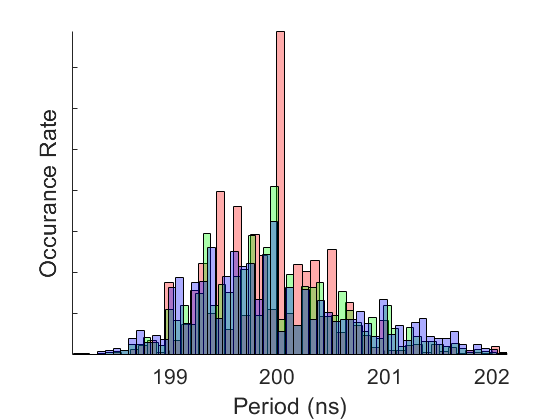
\includegraphics[width=0.8\textwidth]{../dist2}
    \caption[Period distribution at differen divider levels]{Period distribution at differen divider levels.}    
    \label{fig:todo_div}
\end{figure}

\section*{\acs{ADPLL} Use Cases}
As each design was introduced, the most appropriate use cases for that particular \ac{ADPLL} were suggested. \ac{ADPLL} networks can be used in a number of roles, from modelling system dynamics or the refinement of behavioural simulation models to the validation, verification and testing of potential \ac{ASIC} based networks (Zianbetov \& Shan) to the design of other hardware for the purposes of network performance improvement or control, however, some architectures of \ac{ADPLL} are more suited to particular roles than others.

As mentioned when \ac{FPGA} clocked designs were introduced, their configurability makes them particularly suited to the validation and verification of designs destined for use in \acp{ASIC}, as was the case with Zianbetov and Shan \cite{zianbetov2013phd,shan2014phd}. In contrast to the \ac{RO} based designs, in which configurability is more more restricted, it is possible to replicate the resolution, centre frequencies and other \ac{ADPLL} characteristics of the design requiring verification at a scaled down frequency. This can be carried out at large division ratios, where the \ac{FPGA} clock period is not a restricting factor, such as the $50~\si{kilo\hertz}$ centre frequency used by Zianbetov and Shan. In order to reduce the frequency to this extent with inverters over $30$ thousand would be required, introducing the potential for even greater variation in centre frequencies due to implementation. The other issue arising out of this number of inverters is the floorspace of the \ac{FPGA} that would be consumed implementing just one \ac{RO}, in the case of the Xilinx \acl{Nexys} and extrapolating based on the resource usage of the \acp{RO} implemented, a single oscillator would consume half the look-up tables available, eliminating the possibility of a network.

While the \ac{FPGA} based designs feature characteristics making them particularly suitable for use as a validation tool, their performance in a network reduces their suitability for the refinement of software based simulations, or in the analysis of new control or performance enhancement tools. Referring back to Table \ref{table:2x2perf}, \ac{C2C} jitter is significantly greater than the inverter based designs, and a large degree of skew is present making this design non-ideal for these purposes. In particular, as seen with the increase to a 3x3 network, this skew becomes an issue that limits the network size.

Figure \ref{fig:dists}, which demonstrated the impact of period distribution, highlights a second major unrealistic behaviour present in \ac{FPGA} clocked \ac{ADPLL} designs, as \iac{ASIC} destined design will not exhibit this identical linear period distribution. While \ac{ADPLL} 2 will feature a large degree of variation due to implementation differences, these differences are only present in the \ac{RO} not the \ac{PFD}. As testing Designs 2 \& 3 has shown, in particular the results displayed in Table \ref{table:2x2perf}, apart from a larger skew, the jitter performance is quite similar, meaning that the extra complexity of inverter based \ac{PFD} is not required in order to achieve as accurate behaviour as can be achieved in this environment. The implementation based variation of the detector step manifests itself as an increase in the jitter across all network modes, as would be expected, compared to the \ac{FPGA} based design.

Accordingly, if the aim of this platform is the enhancement of a model, the validation of theoretical results, or analysing the performance of new control or performance enhancement hardware the \ac{RO} based designs are idea for this purpose. Two members of the research team here in \acs{UCD}, Eugene Koskin and Pierre Bisiaux, have been using \iac{ADPLL} with the same architecture as Design 3 for these purposes.

